\chapter{Experimental validation} % (fold)
\label{cha:experimental_validation}
    In this chapter I'll show and discuss the results obtained by the tests of the standard and fastflow
    versions of the program implementing the watermarking project. As explained in chapter
    \ref{cha:performance_modeling}, I've considered the most known measures from the parallel/distributed
    computing point of view. Figure \ref{fig:performances} represents the progress of every measure compared
    to the parallelism degree. In order to verify that the models defined in chapter
    \ref{cha:performance_modeling} can be used to represent the evolution of the performances, I've used the
    data returned by every execution's output. You can see an example of output in appendix
    \ref{sec:how_to_run_the_program}.
    \section{Completion time} % (fold)
    \label{sec:completion_time}
        Figure \ref{fig:completion_time_standard} and \ref{fig:completion_time_fastflow} shows the progression
        for the completion time compared to the parallelism degree. As we can see, both for the standard program
        and the fastflow program, there is a initial decreasing of the completion time, that suddendly remains
        quite stable for the remaining part of the plots. The fastflow version of the program executed on my
        laptop, a MacBook Pro, exposes a strange behavior, in which we can see an increasing of the completion
        time compared to the parallelism degree.
        \subsection{Sequential model's validation} % (fold)
        \label{sub:sequential_model_s_validation}
            Observing the completion time for the sequential execution, we can see that the
            reported result follows the model described by equation \ref{eq:completion_time_sequential}. Having
            the time taken to process an image represented by equation \ref{eq:sequential}, the summation over
            the number of processed images gives us the total completion time taken by the sequential execution
            of the program.
        % subsection sequential_model_s_validation (end)
        \subsection{Parallel model's validation} % (fold)
        \label{sub:parallel_model_s_validation}
            As stated before, the completion time for the parallel execution is characterized by an initial
            decreasing and suddendly by a stabilization. As explained in chapter
            \ref{cha:implementation_structure_and_implementation_details}, this is because the functions for
            loading and saving images (taken from \cite{cimg}) both represents a bottleneck for
            the overall computation. We can use the results provided by the various executions to assume that
            the parallel execution of the program follows the model described by equation
            \ref{eq:completion_time_parallel}, with the loading time, and the delay, representing the
            bottleneck for this kind of computation.
        % subsection parallel_model_s_validation (end)
    % section completion_time (end)
    \section{Speedup} % (fold)
    \label{sec:speedup}
        Figure \ref{fig:speedup_standard} and \ref{fig:speedup_fastflow} shows the progression for the speedup
        compared to the parallelism degree. As we can see, for the standard versions of the program, there is a
        initial increasing in the speedup compared to the parallelism degree, which suddendly remains stable
        for both the machines. For the fastflow version, as for the completion time, the execution on my laptop
        presents a strange behavior. The standard version of the program, as we can see, runs twice as faster
        as the sequential one on the department's machine starting from parallelism degree $2$, while on my
        laptop the speedup is approximately $1.5$. The fastflow version shows a slightly worse behavior on the
        department's machine.
    % section speedup (end)
    \section{Scalability} % (fold)
    \label{sec:scalability}
        Figure \ref{fig:scalability_standard} and \ref{fig:scalability_fastflow} shows the progression for the
        scalability compared to the parallelism degree. The standard version of the program executed on my
        laptop presents a mean scalability eguals to $1.2$, while it is slightly higher on the department's
        machine, with a value of $1.6$.
    % section scalability (end)
    \section{Efficiency} % (fold)
    \label{sec:efficiency}
        Figure \ref{fig:efficiency_standard} and \ref{fig:efficiency_fastflow} shows the progression for the
        efficiency compared to the parallelism degree.
    % section efficiency (end)
    \begin{figure}
        \centering
        \begin{subfigure}{0.33\textwidth}
            \resizebox{\textwidth}{!}{
                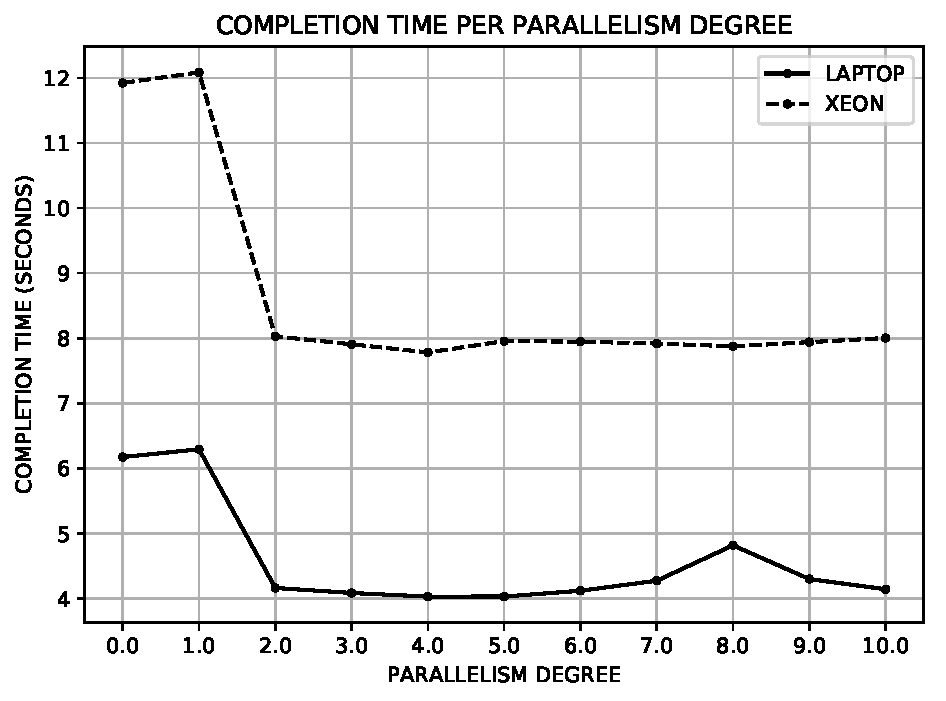
\includegraphics{imgs/completion_time_standard.pdf}
            }
            \caption{Standard}
            \label{fig:completion_time_standard}
        \end{subfigure}
        \begin{subfigure}{0.33\textwidth}
            \resizebox{\textwidth}{!}{
                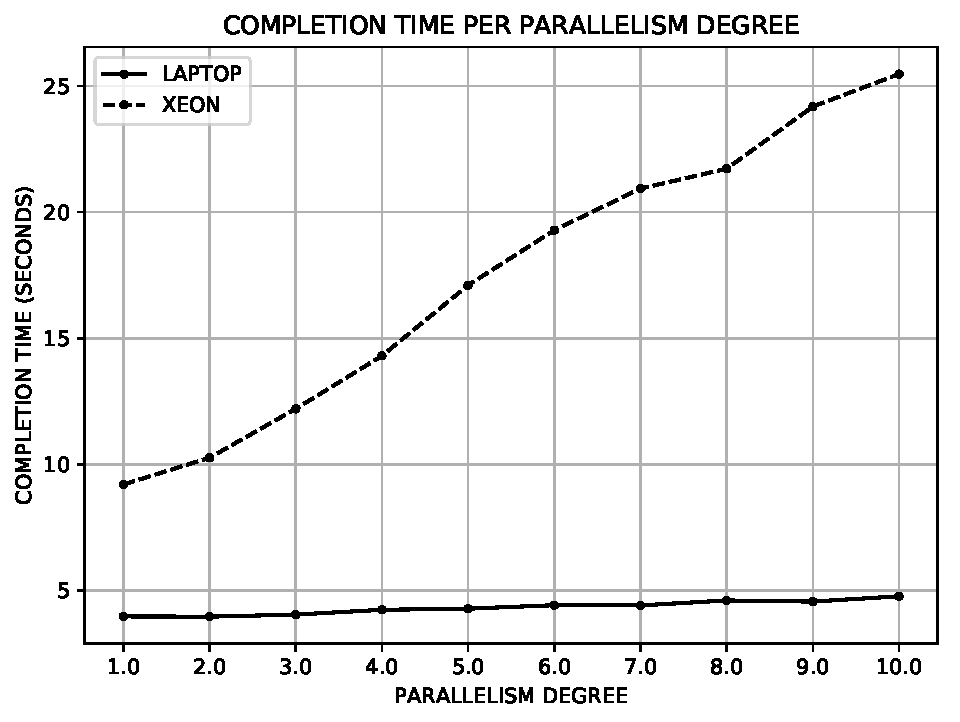
\includegraphics{imgs/completion_time_fastflow.pdf}
            }
            \caption{Fastflow}
            \label{fig:completion_time_fastflow}
        \end{subfigure}
        \begin{subfigure}{0.33\textwidth}
            \resizebox{\textwidth}{!}{
                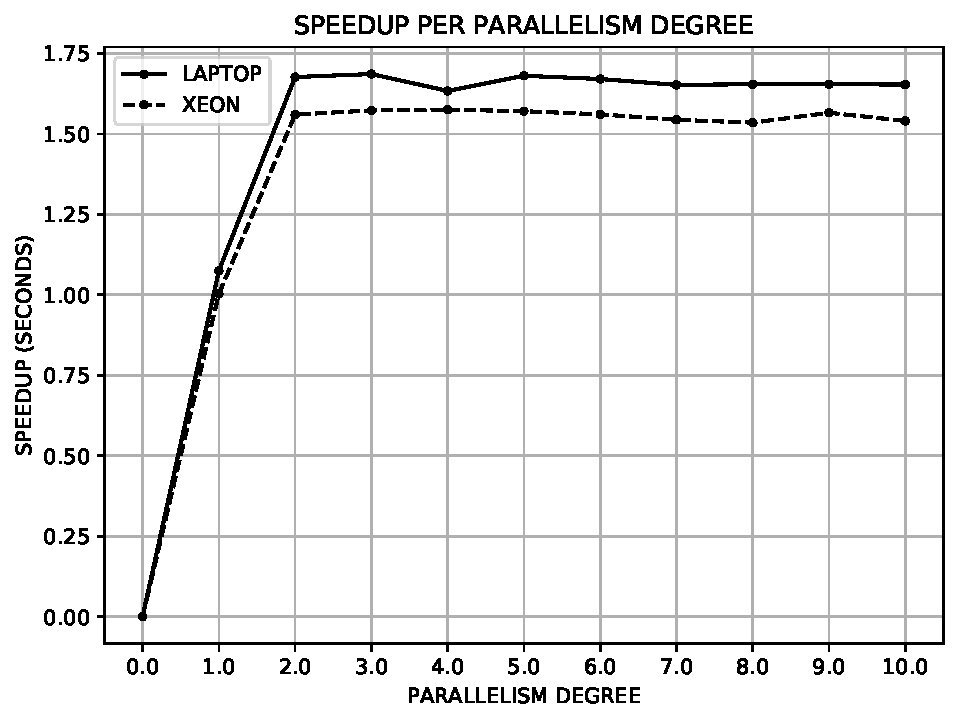
\includegraphics{imgs/speedup_standard.pdf}
            }
            \caption{Standard}
            \label{fig:speedup_standard}
        \end{subfigure}
        \begin{subfigure}{0.33\textwidth}
            \resizebox{\textwidth}{!}{
                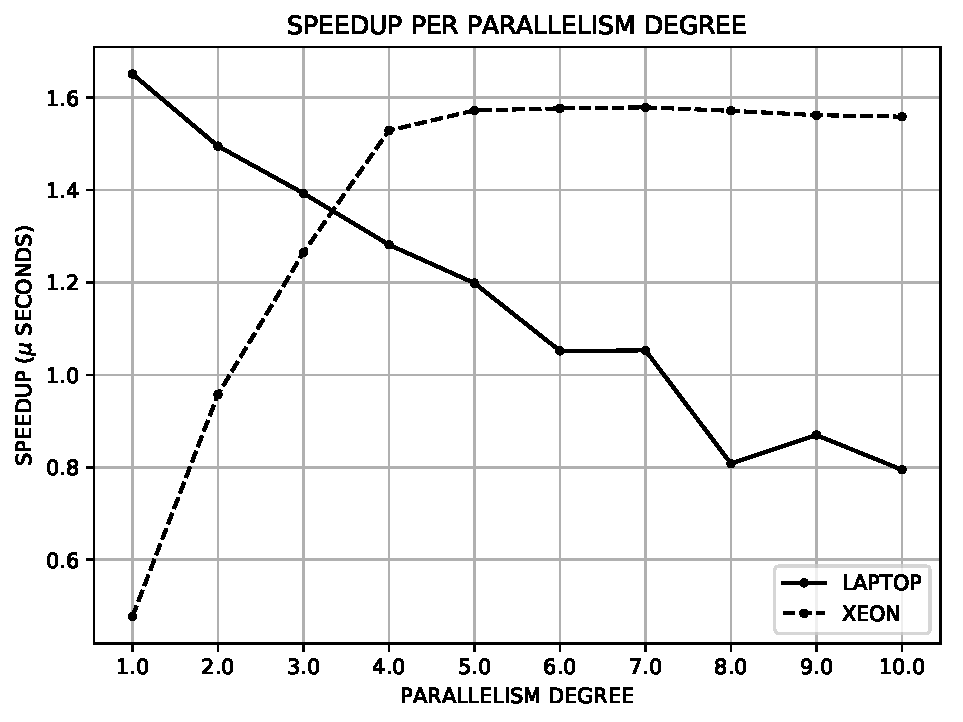
\includegraphics{imgs/speedup_fastflow.pdf}
            }
            \caption{Fastflow}
            \label{fig:speedup_fastflow}
        \end{subfigure}
        \begin{subfigure}{0.33\textwidth}
            \resizebox{\textwidth}{!}{
                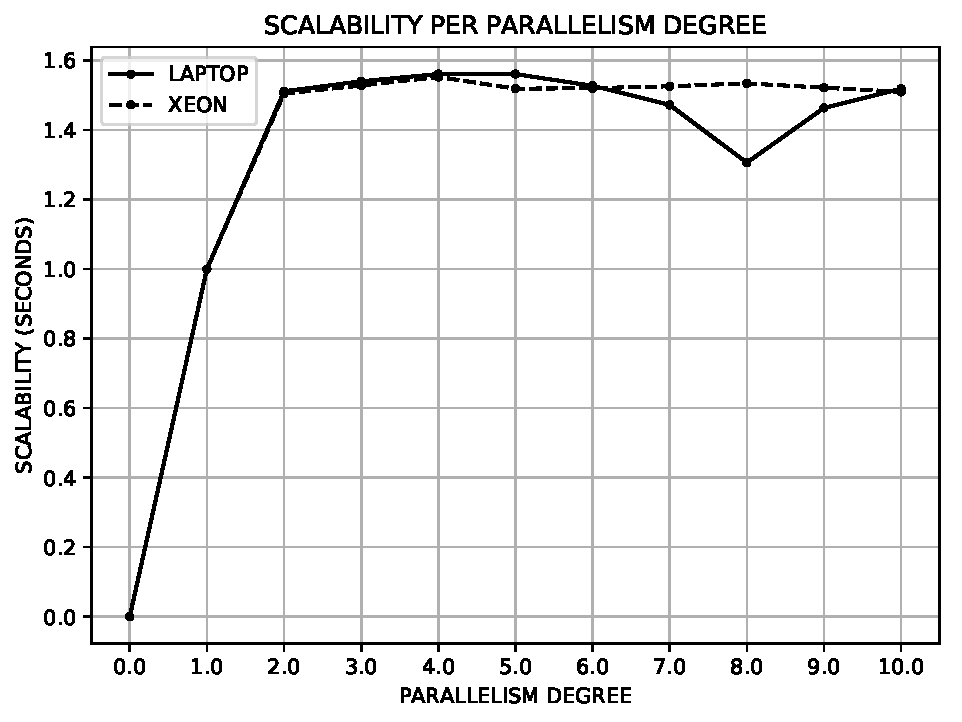
\includegraphics{imgs/scalability_standard.pdf}
            }
            \caption{Standard}
            \label{fig:scalability_standard}
        \end{subfigure}
        \begin{subfigure}{0.33\textwidth}
            \resizebox{\textwidth}{!}{
                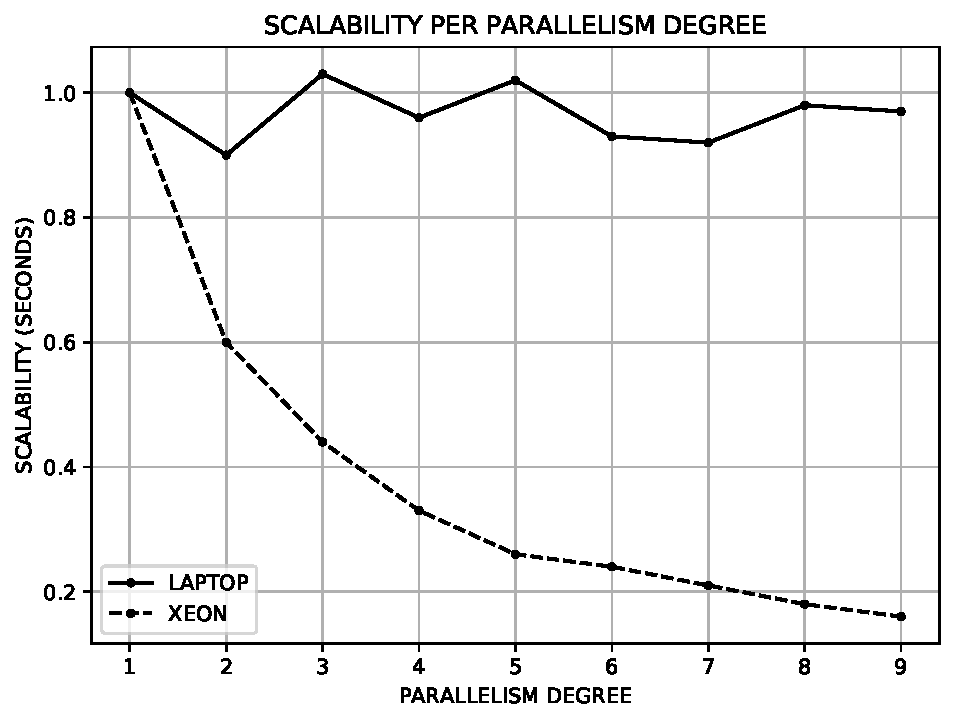
\includegraphics{imgs/scalability_fastflow.pdf}
            }
            \caption{Fastflow}
            \label{fig:scalability_fastflow}
        \end{subfigure}
        \begin{subfigure}{0.33\textwidth}
            \resizebox{\textwidth}{!}{
                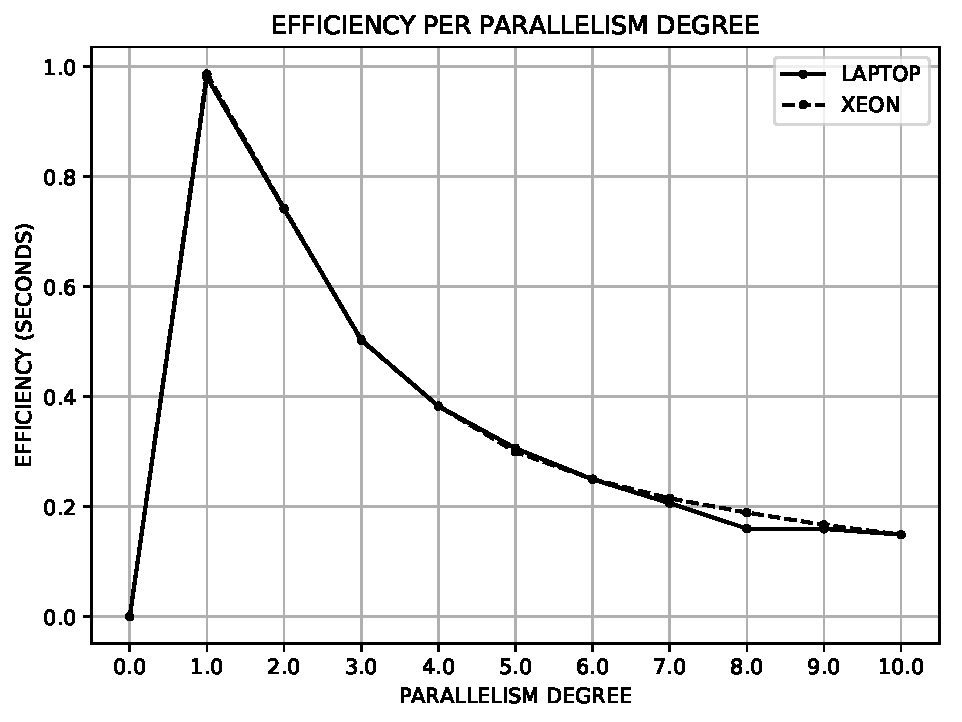
\includegraphics{imgs/efficiency_standard.pdf}
            }
            \caption{Standard}
            \label{fig:efficiency_standard}
        \end{subfigure}
        \begin{subfigure}{0.33\textwidth}
            \resizebox{\textwidth}{!}{
                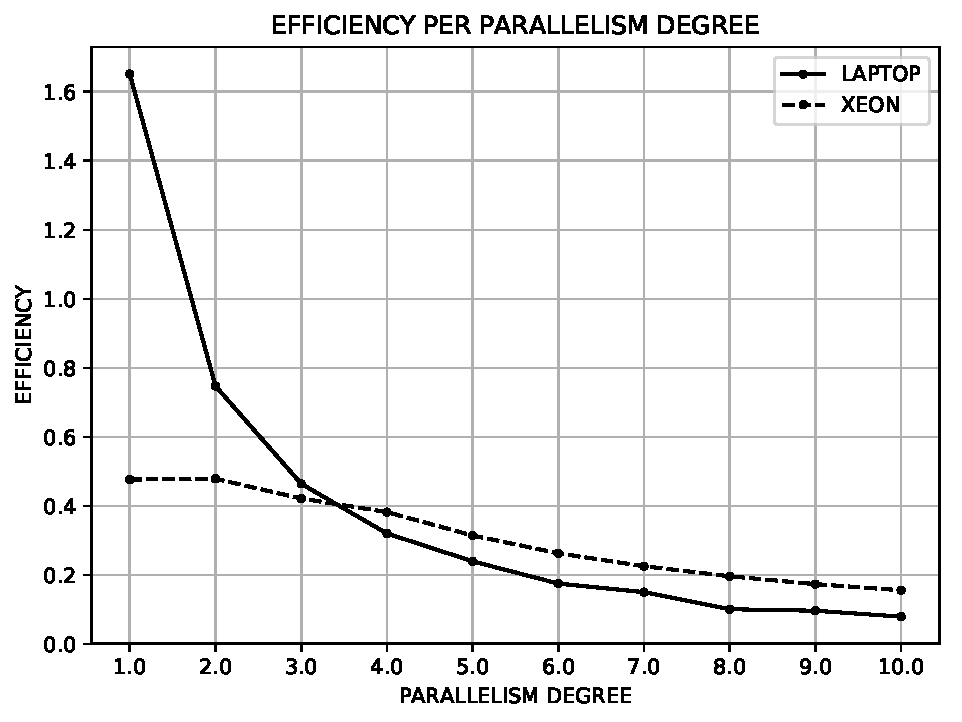
\includegraphics{imgs/efficiency_fastflow.pdf}
            }
            \caption{Fastflow}
            \label{fig:efficiency_fastflow}
        \end{subfigure}
        \caption{Plots of the measures described in chapter \ref{cha:performance_modeling}. The standard
        version was tested with a parallelism degree that ranges from $0$ to $10$, while the fastflow one was
        tested with a parallelism degree that ranges from $1$ to $10$. The solid line represents an execution
        on my laptop, while the dotted line represents an execution on the department's machine. On every
        plot's x-axis we can see the progression of the parallelism degree, where the $0$
        value in the program's standard execution represents the sequential execution, while on every plot's
        y-axis we can see the value of the measure for a particular parallelism degree.}
        \label{fig:performances}
    \end{figure}
    \newpage
    \pagenumbering{Roman}
    \setcounter{page}{2}
% chapter experimental_validation (end)
